\documentclass[10pt,letterpaper]{article}

\usepackage{amsmath}
\usepackage{tikz}
\usepackage{hyperref}

\newcommand{\volume}{{\ooalign{\hfil$V$\hfil\cr\kern0.08em--\hfil\cr}}}

\author{Thaddeus Hughes \\ hughes.thad@gmail.com \\ thaddeus-maximus.github.io}
\date{\today}
\title{Adiabatic Model of a Pneumatic Cylinder}



\begin{document}
	\maketitle
	
	\begin{abstract}
		There are some basic models for pneumatic cylinders that result in modeling cylinders as constant-force devices, or nearly so. This is a rough first pass at creating a model that is a little more sophisticated. This model assumes that the air in the cylinder is adiabatic; that is, no heat transfer takes place. This model will be a differential equation intended to be used in conjunction with a numerical DE solver due to the non-linear nature of many conditions.
		
		Pneumatic pistons can be used for many scenarios- they can act as quick stops, can push or pull heavy loads, or can be configured to quickly launch objects. Depending on the nature of the system, they can behave quite differently, and this model may capture more of the underlying physics that affects these various use cases.
	\end{abstract}
	
	\section*{System Definition}
	
	We will analyze the open system that is the air contained within a pneumatic cylinder, plus the air in the hose leading up to it (inclusion of the hose will become of crucial importance and will be evident later on).
	\begin{center}
	\begin{tikzpicture}[x=1.0in,y=1.0in]
		\draw[->] (-0.5,0)--(-0.1,0) node[pos=0, left]{$P_{in}$, $\dot{\volume}_{in}$, $T_{in}$};
		
		\draw[] (0.3,-0.1)--(0,-0.1)--(0,0.1)--(0.3,0.1)--(0.3,0.5)--(1.2,0.5)--(1.2,-0.5)--(0.3,-0.5)--cycle;
		\node (state) [text width=0.4] at (0.65,0) {$m_s$ \\ $P_s$ \\ $\volume_s$ \\ $T_s$};
		\draw[->] (1.0, 0.6)--(1.4, 0.6) node[pos=0.5, above] {$v$, $x$};
		%\draw[->] (1.9,0)--(1.4,0) node[pos=0, above] {$F = P_{atm} A$};
	\end{tikzpicture}
	\end{center}
	
	Air at pressure $P_{in}$ and temperature $T_{in}$ enters the cylinder at rate $\dot{\volume}_{in}$.
	It mixes with air in the cylinder ($m_s$, $\volume_s$) and is assumed to become of uniform pressure and temperature $P_s$ and $T_s$.
	
	The piston ram is moving at velocity $v$ and with position $x$. $x$ is zero when the cylinder is bottomed out (no air in the cylinder). 
	
	\begin{center}
	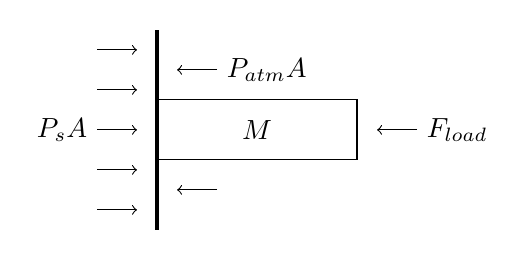
\begin{tikzpicture}[x=1.0in,y=1.0in]
		\draw[ultra thick] (0,-0.5)--(0,0.5);
		\draw[] (0,-0.15)--(0,0.15)--(1,0.15)--(1,-0.15)--cycle;
		
		\node (ctr) [] at (0.5,0) {$M$};
		
		\draw[->] (-0.3,0)--(-0.1,0) node[pos=0,left]{$P_s A$};
		\draw[->] (-0.3,0.2)--(-0.1,0.2); \draw[->] (-0.3,0.4)--(-0.1,0.4); \draw[->] (-0.3,-0.2)--(-0.1,-0.2); \draw[->] (-0.3,-0.4)--(-0.1,-0.4);
		
		\draw[->] (1.3,0)--(1.1,0) node[pos=0,right]{$F_{load}$};
		\draw[->] (0.3,0.3)--(0.1,0.3) node[pos=0,right]{$P_{atm} A$};
		\draw[->] (0.3,-0.3)--(0.1,-0.3);
	\end{tikzpicture}
	\end{center}
	
	The cylinder itself is considered to have a mass $M$ and sees the cylinder pressure, a resistive force $F_{load}$, and atmospheric pressure.
	
	\section*{Conservation Principles In The Cylinder}
	
	First, let's apply conservation of mass to the air.
	
	\begin{align}
		\frac{d}{dt} m_{sys} &= \sum_{+ in} \dot{m} \nonumber
	\end{align}\begin{align} \label{eq:ddt_m}
		\frac{d}{dt} m_s &= \dot{m}_{in}
	\end{align}
	
	We can use the ideal gas law $P \volume = m R T$ to write this in terms of knowns.
	\begin{align}
		\dot{m}_{in} = \frac{P_{in} \dot{\volume}_{in}}{R T_{in}} \nonumber
	\end{align}
	
	We'll assume that the primary flow restriction comes from the tube. We can use an equation derived from \href{https://www.engineeringtoolbox.com/pressure-drop-compressed-air-pipes-d_852.html}{this empirical pipe flow equation in The Engineering ToolBox}.
	
	\begin{align} 
		\dot{\volume} = 0.0197862 (d_{tube}^5 [P_{in}-P_{atm}] [P_{in}-P_{s}]/L_{tube})^{20/37} \nonumber
	\end{align}
	(Assuming units of $Pa$, $m$, and $m^3/s$)
	
	\begin{align} \label{eq:sup_mdot}
		\dot{m}_{in} = \frac{0.0197862}{R T_{in}} (d_{tube}^5 [P_{in}-P_{atm}] [P_{in}-P_{s}]/L_{tube})^{20/37}
	\end{align}
	
	Now, let's apply conservation of energy.
	
	\begin{align}
		\frac{d}{dt} E_{sys} = \sum \dot{Q}_{in} + \sum \dot{W}_{in} + \sum_{+in} \dot{m} (v^2/2 + gz + h) \nonumber
	\end{align}
	
	We will assume:
	\begin{itemize}
		\item The energy of the system is entirely thermal; $E_sys$ = $m_s u(T)$
		\item No heat transfer; $\dot{Q}_{in} = 0$
		\item Work is out of the system, defined by the pressure of the system and velocity of the ram; $\dot{W}_{in} = - \vec{F} \cdot \vec{v} = - P_s A v$
		\item Mass transfer into the system has negligible velocity ($v$) and head height ($gz$), leaving only enthalpy $h(T)$.
	\end{itemize}		
	
	\begin{align}
		\frac{d}{dt} [m_s u(T)] = - P_s A v + \dot{m}_{in} h(T_{in}) \nonumber
	\end{align}
	
	The derivative here is quite ugly, since both the mass and temperature of the system are changing. However, it can be broken up with the product rule ($\frac{d}{dt}[xy] = y \frac{dx}{dt} + x \frac{dy}{dt}$).
	
	\begin{align} 
		m_s \frac{d u(T_s)}{dt} + u(T_s) \frac{d m_s}{dt} = - P_s A v + \dot{m}_{in} h(T_{in}) \nonumber \\
		m_s \frac{d u(T_s)}{dt} = \dot{m}_{in} h(T_{in}) - P_s A v - u(T_s) \frac{d m_s}{dt} \nonumber
	\end{align}
	
	Recognizing that $u(T)$ and $h(T)$ can be approximated as $u(T) = c_p T$ and $h(T) = c_v T$, we can then solve the equation for $\frac{dT_s}{dt}$.
	
	\begin{align} \label{eq:ddt_T}
		\frac{d T_s}{dt} = \frac{ \dot{m}_{in} c_v T_{in} - P_s A v - c_p T_s \dot{m}_{in} }{c_p m_s}
	\end{align}
	
	All of these are knowns or states aside from $P_s$, which can be determined with the ideal gas law, and the modeling of the system volume as based on cylinder extension, crossectional area, and initial (i.e. hose) dead volume.
	
	\begin{align}
		P_s = \frac{m_s R T_s}{\volume_s} \nonumber
	\end{align}\begin{align} \label{eq:sup_P}
		P_s = \frac{m_s R T_s}{\volume_{dead} + x A}
	\end{align}
	
	\section*{Conservation Principles on the Piston}
	
	We can simply apply conservation of linear momentum to the piston.
	
	\begin{align}
		\frac{d}{dt} P_{sys}= \sum F + \sum \dot{m} v \nonumber
	\end{align}
	
	We will assume:
	\begin{itemize}
		\item No mass transfer in this system, so $\frac{d}{dt} P_{sys} = M \frac{dv}{dt}$ and $\dot{m}=0$
		\item The forces acting on the piston are the cylinder pressure, atmospheric pressure, and the external load.
	\end{itemize}
	
	\begin{align}
		M \frac{dv}{dt} &= P_s A - P_{atm} A - F_{load} \nonumber
	\end{align}\begin{align}  \label{eq:ddt_v}
		\frac{dv}{dt} &= \frac{(P_s - P_{atm}) A - F_{load}}{M}
	\end{align}
	
	We are also interested in the position of the piston.
	
	\begin{align} \label{eq:ddt_x}
		\frac{dx}{dt} = v
	\end{align}
	
	\section*{Limiting the Model}
	In review we have:
	
	\begin{itemize}
		\item A model for rate of change of $m_s$
		\item A model for rate of change of $T_s$
		\item Supporting equation for cylinder pressure $P_s$
		\item Supporting equation for massflow into cylinder $\dot{m}$
		\item A model for velocity $v$
		\item A model for position $x$
	\end{itemize}
	
	We simply now need initial conditions, "bumper" conditions, and termination criteria.
	
	We will assume the initial temperature $T_s$ will be set to that of the input gas $T_{in}$. (This may seem like it would negate all the point of this model, but recall that when gases expand/contract, they change pressure)
	
	\begin{align} \label{eq:ic_T}
		T_s(t=0) = T_{in}
	\end{align}
	
	The initial mass of cylinder air can be found with the ideal gas law, assuming we start at atmospheric pressure (wholly unpressurized)
	
	\begin{align} \label{eq:ic_m}
		m_s(t=0) = \frac{P_{atm} L_{tube} \frac{\pi}{4} d_{tube}^2}{R T_s(t=0)}
	\end{align}
	
%	There's an interesting edge case that our model doesn't look at, and that's when we overfill the cylinder. Air can't keep coming into our cylinder. An orifice model may be more appropriate, but let's just say that if the cylinder pressure is greater than the input pressure, no more air can be added.
	
%	\begin{equation} \label{eq:bump_pres}
%		\mbox{if } P_s > P_{in} \mbox{ then } \dot{m}_{in} = 0
%	\end{equation}	 
	
	Assume the piston starts from rest.
	
	\begin{align} \label{eq:ic_x}
		x(t=0) &= 0
	\end{align}\begin{align}\label{eq:ic_v}
		v(t=0) &= 0
	\end{align}
	
	And that the piston cannot go past its endstops at $x=x_f$ or $x=0$.
	
	\begin{align} \label{eq:bump_end}
		\mbox{if } x \geq x_f &\mbox{ then } x = x_f, v \leq 0
	\end{align}\begin{align}\label{eq:bump_start}
		\mbox{if } x \leq 0   &\mbox{ then } x = 0, v \geq 0  
	\end{align}
		
	We will terminate our simulation when we reach the endstop and fully pressurize.
	
	\begin{align} \label{eq:term}
		\mbox{terminate simulation if } x \geq x_f \mbox{ and } P_s \geq P_{in}
	\end{align}
	
	\section*{The Full Model}
	
	\begin{align}
		\dot{m}_{in} &= \frac{0.0197862}{R T_{in}} (d_{tube}^5 [P_{in}-P_{atm}] [P_{in}-P_{s}]/L_{tube})^{20/37} \tag{\ref{eq:sup_mdot}} \\
		P_s &= \frac{m_s R T_s}{L_{tube} \frac{\pi}{4} d_{tube}^2 + x A} \tag{\ref{eq:sup_P}} \\			
		\mbox{if } x \geq x_f &\mbox{ then } x = x_f, v \leq 0 \tag{\ref{eq:bump_end}} \\
		\mbox{if } x \leq 0   &\mbox{ then } x = 0, v \geq 0 \tag{\ref{eq:bump_start}} \\
		\frac{d}{dt} m_s &= \dot{m}_{in} \tag{\ref{eq:ddt_m}} \\
		\frac{d T_s}{dt} &= \frac{ \dot{m}_{in} c_v T_{in} - P_s A v - c_p T_s \dot{m}_{in} }{c_p m_s} \tag{\ref{eq:ddt_T}} \\
		\frac{dv}{dt} &= \frac{(P_s - P_{atm}) A - F_{load}}{M} \tag{\ref{eq:ddt_v}} \\
		\frac{dx}{dt} &= v \tag{\ref{eq:ddt_x}} \\
		T_s(t=0)& = T_{in} \tag{\ref{eq:ic_T}} \\
		m_s(t=0) &= \frac{P_{atm} L_{tube} \frac{\pi}{4} d_{tube}^2}{R T_s(t=0)} \tag{\ref{eq:ic_m}} \\
		v(t=0) &= 0 \tag{\ref{eq:ic_v}} \\
		x(t=0) &= 0 \tag{\ref{eq:ic_x}} \\
		\mbox{terminate}& \mbox{ if } x \geq x_f \mbox{ and } P_s \geq P_{in} \tag{\ref{eq:term}}
	\end{align}
	
	There's a lot going on here. But let's do a sanity check and see if there's going to be any issues going forth.
	
	The big equation of interest is $dT_s/dt$.
	\begin{itemize}
		\item If the heat capacity or system mass is larger, then the rate of temperature change decreases (makes sense)
		\item If the cylinder expands ($v > 0$) then the gas expands, lowering the temperature.
		\item Let's focus on this term
			\begin{align}
				  & \dot{m}_{in} c_v T_{in} - c_p T_s \dot{m}_{in} \nonumber \\
				=\ & \dot{m} [c_v T_{in} - c_p T_s] \nonumber \\
				=\ & \dot{m} [h(T_{in}) - u(T_s)] \nonumber \\
				=\ & \dot{m} [u(T_{in}) + P_{in} / \rho_{in} - u(T_s)] \nonumber \\
				\approx \ & \dot{m} [u(T_{in}-T_s) + P_{in} / \rho_{in}] \nonumber
			\end{align}
			
			Recognizing that $T_in > T_s$ since the cylinder is expanding, we see that yes, the massflow into the system corresponds to higher thermal energy transfer, and higher pressure energy transfer.
		\item The mass of the system $m_s$ is in the denominator - if this is zero, the derivative would not exist, so it is imperative that we begin our simulation with some mass (hence, the dead mass $L_{tube} \frac{\pi}{4} d_{tube}^2$ term)
	\end{itemize}
	
	\section*{Implemented Simulation and Examples}
	
	This has been implemented into my \href{http://thaddeus-maximus.github.io/swissarmyengineer/}{Swiss Army Engineer} suite. Here are some example cases, starting with a base case.
	
	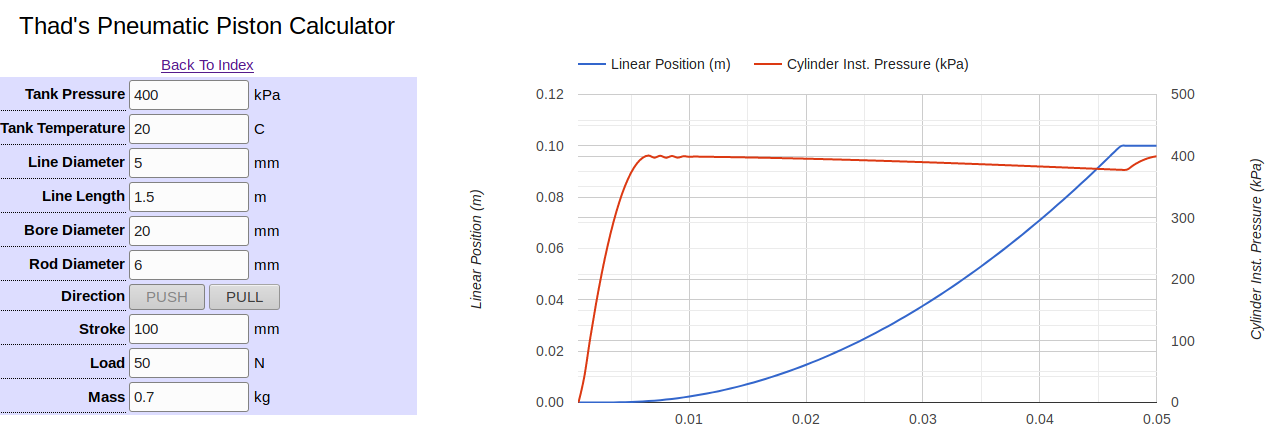
\includegraphics[width=\textwidth]{pneu_case_1.png}
	
	This case has mass, and a load much higher than the mass (simulating, say, a piston pushing on a spring). The results aren't too interesting - air inrushes into the cylinder rather quickly, producing the quadratic position profile you'd expect of a constant-force system.
	
	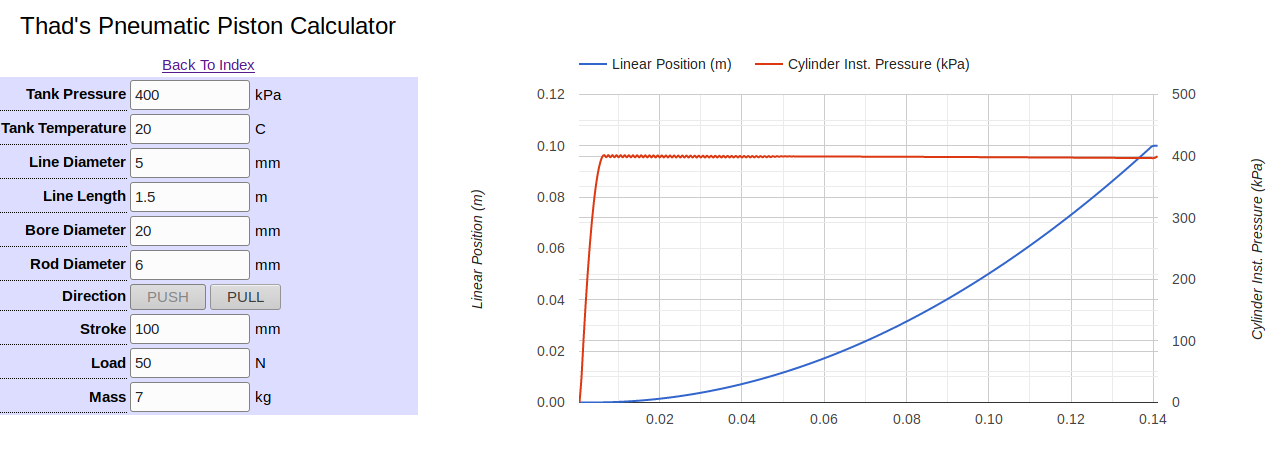
\includegraphics[width=\textwidth]{pneu_case_2.png}
	
	This case increases the mass by ten times. The timescale, accordingly, stretches out, taking much longer to reach its end stop.
	
	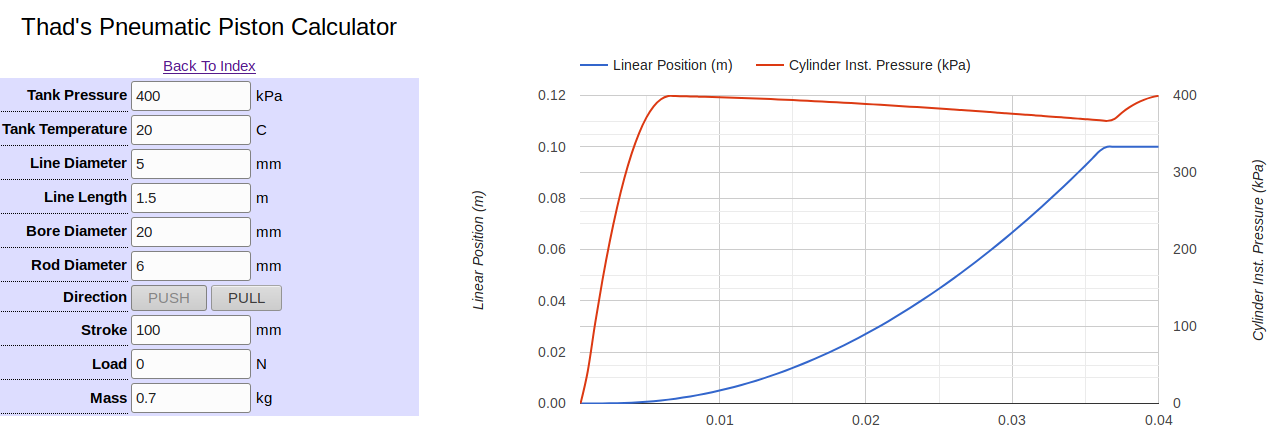
\includegraphics[width=\textwidth]{pneu_case_3.png}
	
	This case removes the load and returns to the lighter system mass, so that this is a purely inertial system. In this case, the piston accelerates like normal, but the cylinder pressure actually begins to decrease as the inertia of the system carries it further forwards. Eventually the hardstop is hit, and at this point the piston can fully pressurize with air.
	
	What happens if we choke it out even further, by shrinking the line diameter?
	
	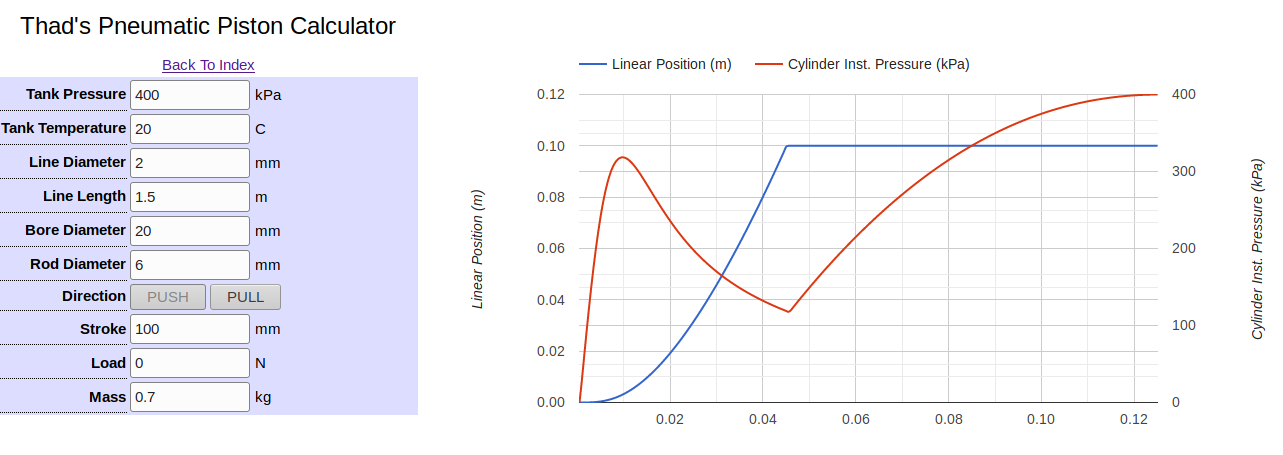
\includegraphics[width=\textwidth]{pneu_case_4.png}
	
	The line diameter here has been shrunk to 2mm. We see this same decayed acceleration as in the previous example, but to a larger degree.
	
	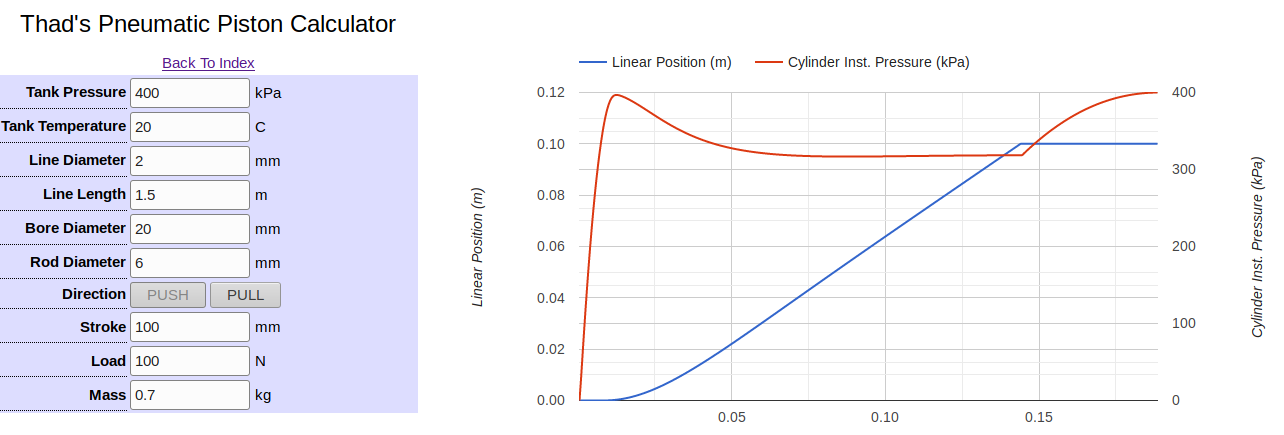
\includegraphics[width=\textwidth]{pneu_case_5.png}
	
	If we add a large load, the position curve becomes linear, as the cylinder has to fight the heavy load and its air supply eventually becomes the limiting factor on speed.
	
	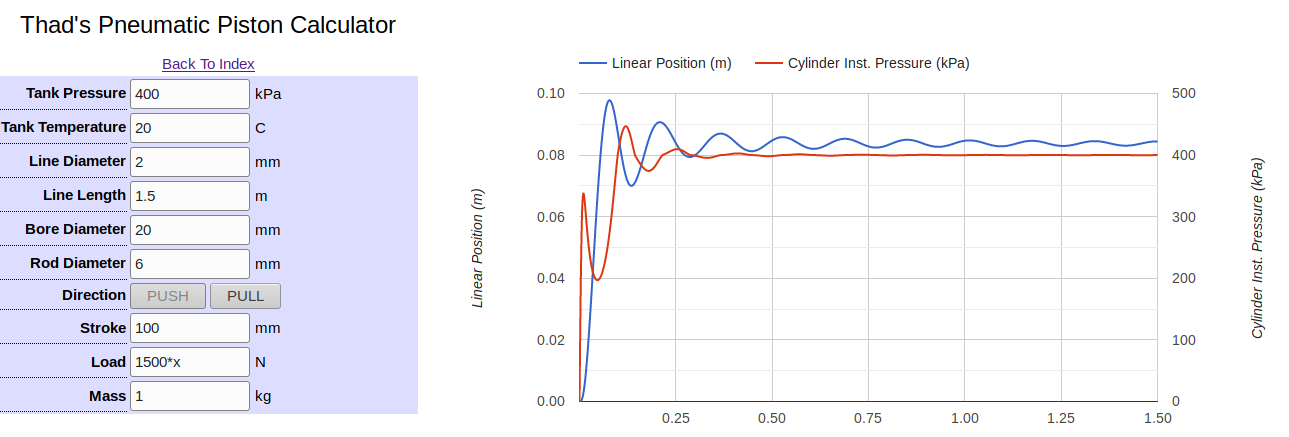
\includegraphics[width=\textwidth]{pneu_case_6.png}
	
	If we make the load an expression, we could model a piston pulling on a spring, giving us this very neat mass-spring system.
	
	\section*{Validation}
		No validation has been performed yet on these models, as I don't have access to the equipment to test them. If anyone wants to perform this testing, it would be very cool!
	
	
\end{document}